\documentclass{beamer}
\usepackage[utf8]{inputenc}
\usepackage[english]{babel}
\usepackage{geometry}
\usepackage{amssymb}
\usepackage{amsfonts}
\usepackage{dsfont}
\usepackage{float}
\usepackage{graphicx}
\usepackage{wrapfig}
\usepackage{mathtools}
\usepackage{bbm}
\usepackage{amsthm}
\usepackage{ifthen}
\usepackage{graphicx}
\usepackage{hyperref}
\usepackage{tcolorbox}
\usepackage[ruled,vlined]{algorithm2e}
\usepackage{tikz}

\usepackage{caption}
\usepackage{subcaption}

%%%%%%%% box %%%%%%%%
\definecolor{mycolor}{rgb}{0.122, 0.435, 0.698}% Rule colour
\makeatletter
\newcommand{\mybox}[1]{%
	\setbox0=\hbox{#1}%
	\setlength{\@tempdima}{\dimexpr\wd0+13pt}%
	\begin{tcolorbox}[colframe=blue,boxrule=0.5pt,arc=4pt,
		left=6pt,right=6pt,top=6pt,bottom=6pt,boxsep=0pt,width=\@tempdima]
		#1
	\end{tcolorbox}
}
%%%%%%%%





\DeclarePairedDelimiter{\ceil}{\lceil}{\rceil}

\newcommand{\ca}[1]{\mathcal{#1}}
\newcommand{\bb}[1]{\mathbb{#1}}
\newcommand{\p}{\mathbb{P}}
\newcommand{\evento}[1]{\left\{ \textit{``#1''} \right\}}
\newcommand{\comillas}[1]{``#1''}
\newcommand{\set}[1]{\left\{#1\right\}}
\newcommand{\parent}[1]{\left(#1\right)}
\newcommand{\parentCuad}[1]{\left[#1\right]}
\newcommand{\borel}{\ca{B}(\bb{R}^d)}
\newcommand{\Rd}{\bb{R}^d}
\newcommand{\R}{\bb{R}}
\newcommand{\infNorm}[1]{||#1||_\infty}
\newcommand{\condExp}[2]{\bb{E}(#1|#2)}
\newcommand{\ind}[1]{\mathbbm{1}_{#1}}
\newcommand{\esp}[1]{\bb{E}\barras{#1}}
\newcommand{\indep}{\rotatebox[origin=c]{90}{$\models$}}
\newcommand{\pe}{$(\Omega, \ca{F}, \p)\ $}
\newcommand{\vc}[1]{\langle #1 \rangle}
\newcommand{\gb}[1]{\overline{\widehat{#1}}}
\newcommand{\barras}[1]{\left| #1 \right|}
\newcommand{\integral}{\int_{t_i}^{t_{i+1}}}
\newcommand{\ug}[1]{\widehat{\ca{U}}_{#1}}
\newcommand{\vg}[1]{\widehat{\ca{V}}_{#1}}
\newcommand{\zg}[1]{\widehat{\ca{Z}}_{#1}}
\newcommand{\norm}[1]{\left\lVert#1\right\rVert}
\newcommand{\X}{\ca{X}}
\newcommand{\xscheme}[1]{X_{t_{#1}}^{\pi}}
\newcommand{\prom}[1]{\langle #1 \rangle}


%\usetheme{Darmstadt default}
\usetheme{Copenhagen}
%\usetheme{Madrid}
%\usecolortheme{beaver}
\usecolortheme{seahorse}
\usefonttheme[onlymath]{serif}
\usefonttheme{structuresmallcapsserif}

\title[Análisis de Datos con Twitter]{Análisis de Datos con Twitter}
\author{Javier Castro M.}
\institute{Universidad De Chile}
\date{\today}


\begin{document}
	\maketitle
	
	\begin{frame}{\textbf{LDA}: \comillas{Latent Dirichlet allocation}}
		LDA es un modelo tipo \textbf{topic modelling}; trata de capturar temas latentes en el texto mediante la calibración de dos parámetros, $\alpha\in [0,1]^{K}$ y $\beta \in [0,1]^{K\times V}$. Donde $K$ es la cantidad de tópicos y $V$ el tamaño del vocabulario. 
		
		\begin{itemize}
			\item Se samplea una distribución sobre tópicos $\theta\sim Dir(\alpha, K)$. Notar que $\sum \theta_i = 1$.
			\item Dado $\theta$, se samplea un tópico $t\sim\theta$.
			\item Dado el tópico $t$, se samplea una palabra $w\sim\beta_{t\cdot}$.
		\end{itemize}
		
		
	\end{frame}

	\begin{frame}{\textbf{LDA}: \comillas{Latent Dirichlet allocation}}
		Para aplicar el LDA podemos usar:
		\begin{itemize}
			\item \texttt{gensim.models.LdaMulticore} (\texttt{broken pipe})
			\item \texttt{gensim.models.LdaModel} 
		\end{itemize}
		Se necesita transformar los textos en \comillas{bag of words}. Los tweets procesados quedan como se ven a continuación:
		
		\begin{figure}[h]
			\centering
			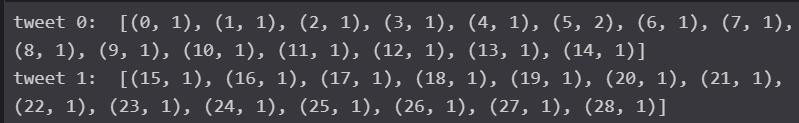
\includegraphics[scale=.5]{../imgs/segunda_avance/bow_tweets_ex.png}
		\end{figure} 
	
		El algoritmo entrega, para cada tópico, una distribución sobre las palabras y una medida llamada \comillas{coherencia}. 
		
	\end{frame}

	\begin{frame}{Resultados}
		Se aplicó el algoritmo a tweets de la cuenta \texttt{@gabrielboric}, a estos se les realizo la limpieza correspondiente.
		
		\begin{itemize}
			\item Resultan $20902$ tweets.
			\item La cantidad de palabras resultantes resultó ser $1853$.
			\item Se buscarán $5$ tópicos.
		\end{itemize}
	\end{frame}

	\begin{frame}{Resultados}
		\begin{figure}[h]
			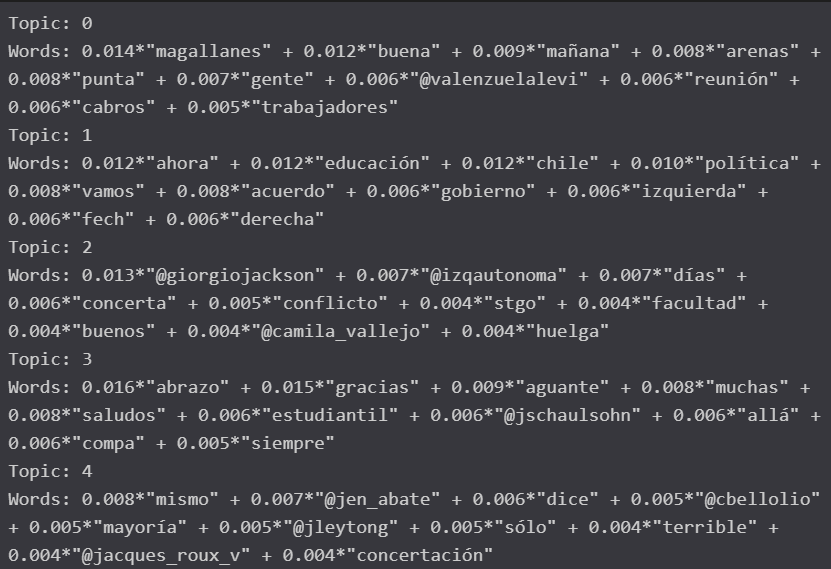
\includegraphics[scale=.4]{../imgs/segunda_avance/boric_5topics_arroba_hash.png}
			\caption{Sin eliminar los @}
		\end{figure}
	\end{frame}

	\begin{frame}{Resultados}
		\begin{figure}[h]
			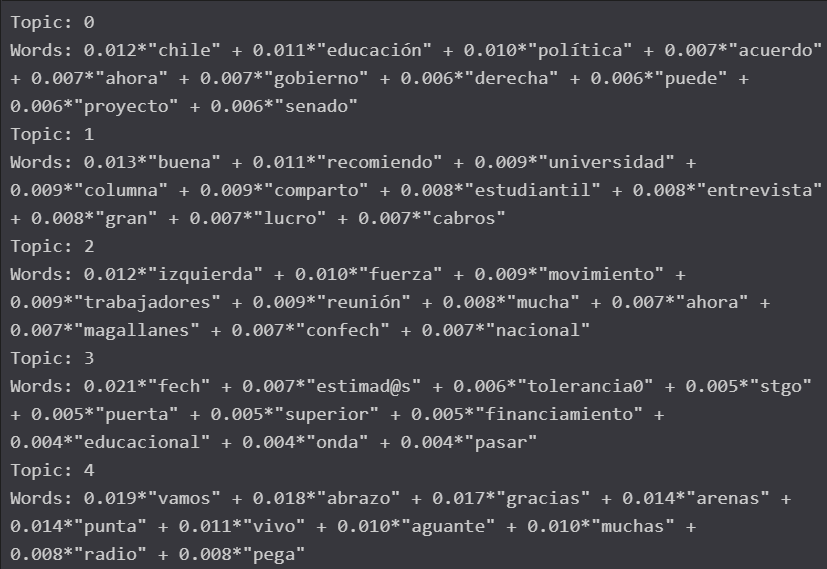
\includegraphics[scale=.4]{../imgs/segunda_avance/boric_5topics.png}
			\caption{Eliminando los @}
		\end{figure}
	\end{frame}


	\begin{frame}{Resultados}
		Se muestra la distribución para el primer tópico.
		\begin{figure}[h]
			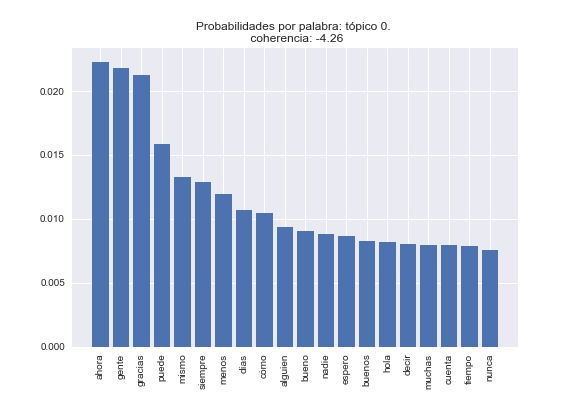
\includegraphics[scale=.4]{../imgs/segunda_avance/boric_barplot0.png}
		\end{figure}
	\end{frame}

	%\begin{frame}{Resultados}
	%	\begin{figure}[h]
	%		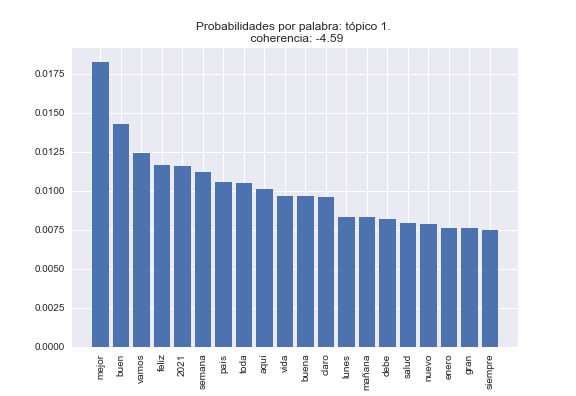
\includegraphics[scale=.4]{../imgs/segunda_avance/boric_barplot1.png}
	%	\end{figure}
	%\end{frame}
	
	\begin{frame}{Resultados}
		Se muestra la coherencia de cada tópico.
		\begin{figure}[h]
			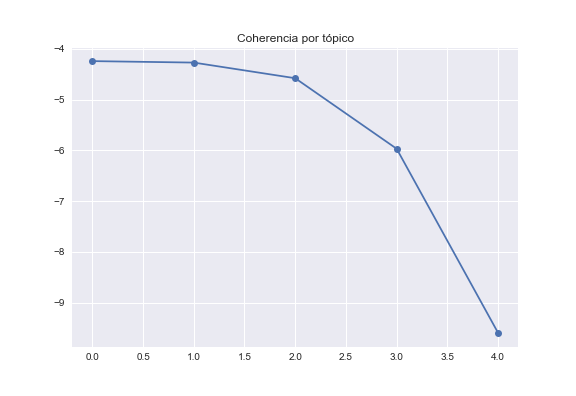
\includegraphics[scale=.4]{../imgs/segunda_avance/boric_topic_coherence.png}
		\end{figure}
	\end{frame}

	\begin{frame}{Ideas y lo que falta}
		\begin{itemize}
			\item Calibrar los hiperparámetros en base a alguna métrica (número de tópicos, $\alpha$ y $\beta$). 
			\item Hacer un limpieza más fina a los tweets (eliminar palabras de muy baja frecuencia, trabajar el problema de palabras mal escritas).
			\item Usar bigrams o similiares.
			\item Quedarse sólo con adjetivos y sustantivos (quizá sólo aplicar esto con un corpus en inglés).
			\item Probar lo mismo con tweets de otros contextos.
		\end{itemize}
	\end{frame}

	\begin{frame}{Bibliografía}
		\begin{itemize}
			\item \textbf{Latent Dirichlet Allocation}, Blei, Ng, Jordan, Journal of Machine Learning Research, 2003.
			\item  \texttt{radimrehurek.com/gensim/models/ldamodel.html}
			\item \textbf{Exploring the Space of Topic Coherence Measures}, Michael Röder, Andreas Both, Alexander Hinneburg, $2015$.
		\end{itemize}
	\end{frame}
	

	\begin{frame}{Fin}
		\centering
		\mybox{Muchas Gracias!}
	\end{frame}

	
	
\end{document}